%\setprocid

% \newcommand{\TestPerfSetup}{Setup and configuration}
% \newcommand{\TestPerfRFPXA}{RF measurements with PXA}
% \newcommand{\TestPerfCCDF}{CCDF measurement}
% \newcommand{\TestPerfFreqS}{Frequency Stability}
% \newcommand{\TestPerfCWPhaseN}{Carrier Phase Noise}
% \newcommand{\TestPerfSpuriousDSN}{Spurious in DSN Band}
% \newcommand{\TestPerfFilterVector}{Data Demodulation Filter Tuning and Vector Analysis}
% \newcommand{\TestPerfBer}{Degraded link test with one X-Band channel}
% \newcommand{\TestPerfSetupBreak}{Tests setup break}

\renewcommand{\reqid}{N/A}
\renewcommand{\procid}{SB1FS-COM-P-013}
\renewcommand{\procname}{Performance Test\xspace}

\section{\procid \ \procname} \label{sec:SB1FS-COM-P-013}


 This section details the test procedures for EWC30 transmitter.
 The figures \ref{fig:data-setup1} and  \ref{fig:data-setup2} show the test setups.
 Solid lines are connections that apply to all downlink tests and dashed 
 lines are connections that change from one test to another.


% \begin{table}[H]
% 	\centering
% 	\footnotesize
% 	\begin{tabular}{|L{3.0cm}|L{13.0cm}|}	
% 		% \hline
% 		% \textbf{Requirement ID} 	& \reqid\\
% 		% \hline
% 		% \textbf{Requirement Statement} & N/A\\ 
% 		\hline
% 		\textbf{Task ID} & \procid{} \\
% 		\hline
% 		\textbf{Task name} & \procname \\
% 		\hline
% 		\textbf{Task description} & In this procedure the EWC30 X-Band transmitter performance test is performed.
		
% Before functional test execution instruments, GS-GSE and CEGSE and configured and interfaces aliveness if performed in case of the last one. 
% Transmitter and Filter ground connections are verified and both RF and base-band DUT interfaces are connected to EGSEs.

% For functional testing the DUT monitoring and control is performed from CEGSE, GS-GSE is prepared to receive data through 
% X-Band interface, Oscilloscope and Signal Analyzer are configured to measure power consumption and RF signals characteristics respectively.

% From CEGSE Data frames will be sent to  EWC30 in order to be modulated and received in GS-GSE. 
% The data received in GS-GSE will be compared with original data. Also RF signals characteristics and signals will be measured.

% \\\hline
% 		\textbf{Task purpose} & Execution of EWC30 functional test. \\
% 		\hline
% 		\textbf{Success criteria} & 			\begin{minipage}[t]{\linewidth}
% 			\begin{itemize}[nosep,after=\strut]
% 		\item Both instruments, CEGSE and GS-GSE, are configured according to procedure and CEGSE interfaces are in good condition.
% DUT telemetry is between expected values.
% 	\item DUT, voltage, current and power consumption in different states meets the expected values.
% 	\item RF signals are under expected values.
% 	\item Data frames received at GS-GSE are the same as those sent from CEGSE.
% 	\item Evidences are collected.
% 				\end{itemize}
% 		\end{minipage}\\
% 		\hline
% 		\textbf{Test sub-cases} & 
% \begin{minipage}[t]{\linewidth}
% 		\begin{itemize}[nosep,after=\strut]
% 		\item \procid{}{-01}: \TestPerfSetup
% 		\item \procid{}{-02}: \TestPerfRFPXA
% 		\item \procid{}{-03}: \TestPerfCCDF
% 		\item \procid{}{-04}: \TestPerfFreqS
% 		\item \procid{}{-05}: \TestPerfCWPhaseN
% 		\item \procid{}{-06}: \TestPerfFilterVector
% 		\item \procid{}{-07}: \TestPerfBer
% 		\item \procid{}{-08}: \TestPerfSpuriousDSN
% 		\item \procid{}{-09}: \TestPerfSetupBreak	
% 		\end{itemize}
% 		\end{minipage}\\
% 		\hline
% 		\textbf{Test Setup} &
% \begin{minipage}[t]{\linewidth}
% 	\begin{itemize}[nosep,after=\strut]
% 		\item \comEgse{}{} to DUT base-band electrical connections according to figure \ref{fig:ewc30_bb} 
% 		\item General setup according to figures \ref{fig:data-setup1} and \ref{fig:data-setup2} for perfomance test.
% 		\end{itemize}
% 	\end{minipage}	
% 		\\ 
% 		\hline
% 		\textbf{Duration} & \begin{minipage}[t]{\linewidth}
% 	\begin{itemize}[nosep,after=\strut]
% 		\item \procid{}{-01}: 120 minutes (TBC)
% 		\item \procid{}{-02}: 240 minutes (TBC)
% 		\item \procid{}{-03}:  minutes (TBC)
% 		\item \procid{}{-04}:  minutes (TBC)
% 		\item \procid{}{-05}:  minutes (TBC)
% 	    \item \procid{}{-06}:  minutes (TBC)
% 	    \item \procid{}{-07}:  minutes (TBC)
% 	    \item \procid{}{-08}:  minutes (TBC)
% 	    \item \procid{}{-09}: minutes (TBC)
% 		\end{itemize}
% 	\end{minipage}
% 	\\ \hline
	
% 	% \textbf{Data sets required} &  \begin{minipage}[t]{\linewidth}
% 	% 	\begin{itemize}[nosep,after=\strut]
% 	% 		\item TM payload file to send (\texttt{SB1-Data-Payload-500MFrames.bin}).
% 	% 		\item \comEgse{}{} PXI configuration file for aliveness (\texttt{INIT\_FILE\_NO\_ALARM\_EWC30.ini}).
% 	% 		\item \comEgse{}{} PXI nominal configuration file for EWC30 (\texttt{INIT\_FILE\_EWC30.ini}).
% 	% 		\item Oscilloscope configuration files in \texttt{osc-config} folder
% 	% 		\item PXA configuration files in \texttt{COMM-SS-EM-PT-PXA-config} folder
% 	% 		\item \texttt{SB1-Data-VC63-10minutes.zip} file
% 	% 		\item GS-GSE M\&C scripts (\texttt{gse\_const.py, gse\_mandc.py, SB1GS-GSE-EM2.0-DemoData-RF-N1.py})
% 	% 			\end{itemize}
% 	% 		\end{minipage}\\
% 	% 	\hline
		
% 				\textbf{Prerequisites} & 
% 		\begin{minipage}[t]{\linewidth}
% 			\begin{itemize}[nosep,after=\strut] 
% 				%\item GS-GSE-FM (R) initialized according to GS-GSE test procedures (\refAD{fm-ver-delta-pro}) or  user manual (\refRD{gs-gse-fm}). 
% 				%\item GS-GSE-FM (R) configured according to Control Configuration Documents (\refAD{gse-cfg-r}) and modified according to report (\refAD{reportFMRMod}).
%  	%\item \comEgse initialized according to \comEgse\xspace user manual (\refAD{cegse}).
% 				\item Execution of procedure SB1FS-COM-D-011 Initialization and dataset deploy.
% 				\item EWC30 and DSN filter mated with the connector savers (RF and BB).
% 				\item EWC30 and DSN filter mounted on \comEgse\xspace metal tray.
% 				\item EWC30 and DSN filter connected to \comEgse\xspace grounding bar.
% 				\item Hardware: The necessary items are shown in the table \ref{tab:req-items} 
% 			\end{itemize} 
% 		\end{minipage}\\
% 		\hline
		
% 	\end{tabular}
% 	%\caption{Procedure \procid{} \ description. } \label{tb:\procid{}-003}
% \end{table}

% %% Test Setup
% \begin{figure}[H]
% 	\centering
% 	  \includegraphics[width=.9\linewidth]{figuras/CEGSE_EWC30_con.png}  
% 	  \caption{EWC30 BB Connections.}
% 	\label{fig:ewc30_bb}
% \end{figure}


\begin{figure}[H]\centering
	\includegraphics[width=1\linewidth]{figuras/EWC30-PXA-Setup1.png}  
	\caption{EWC30 Transmissions Test Setup }
  \label{fig:data-setup1}
\end{figure}

\begin{figure}[H]\centering
	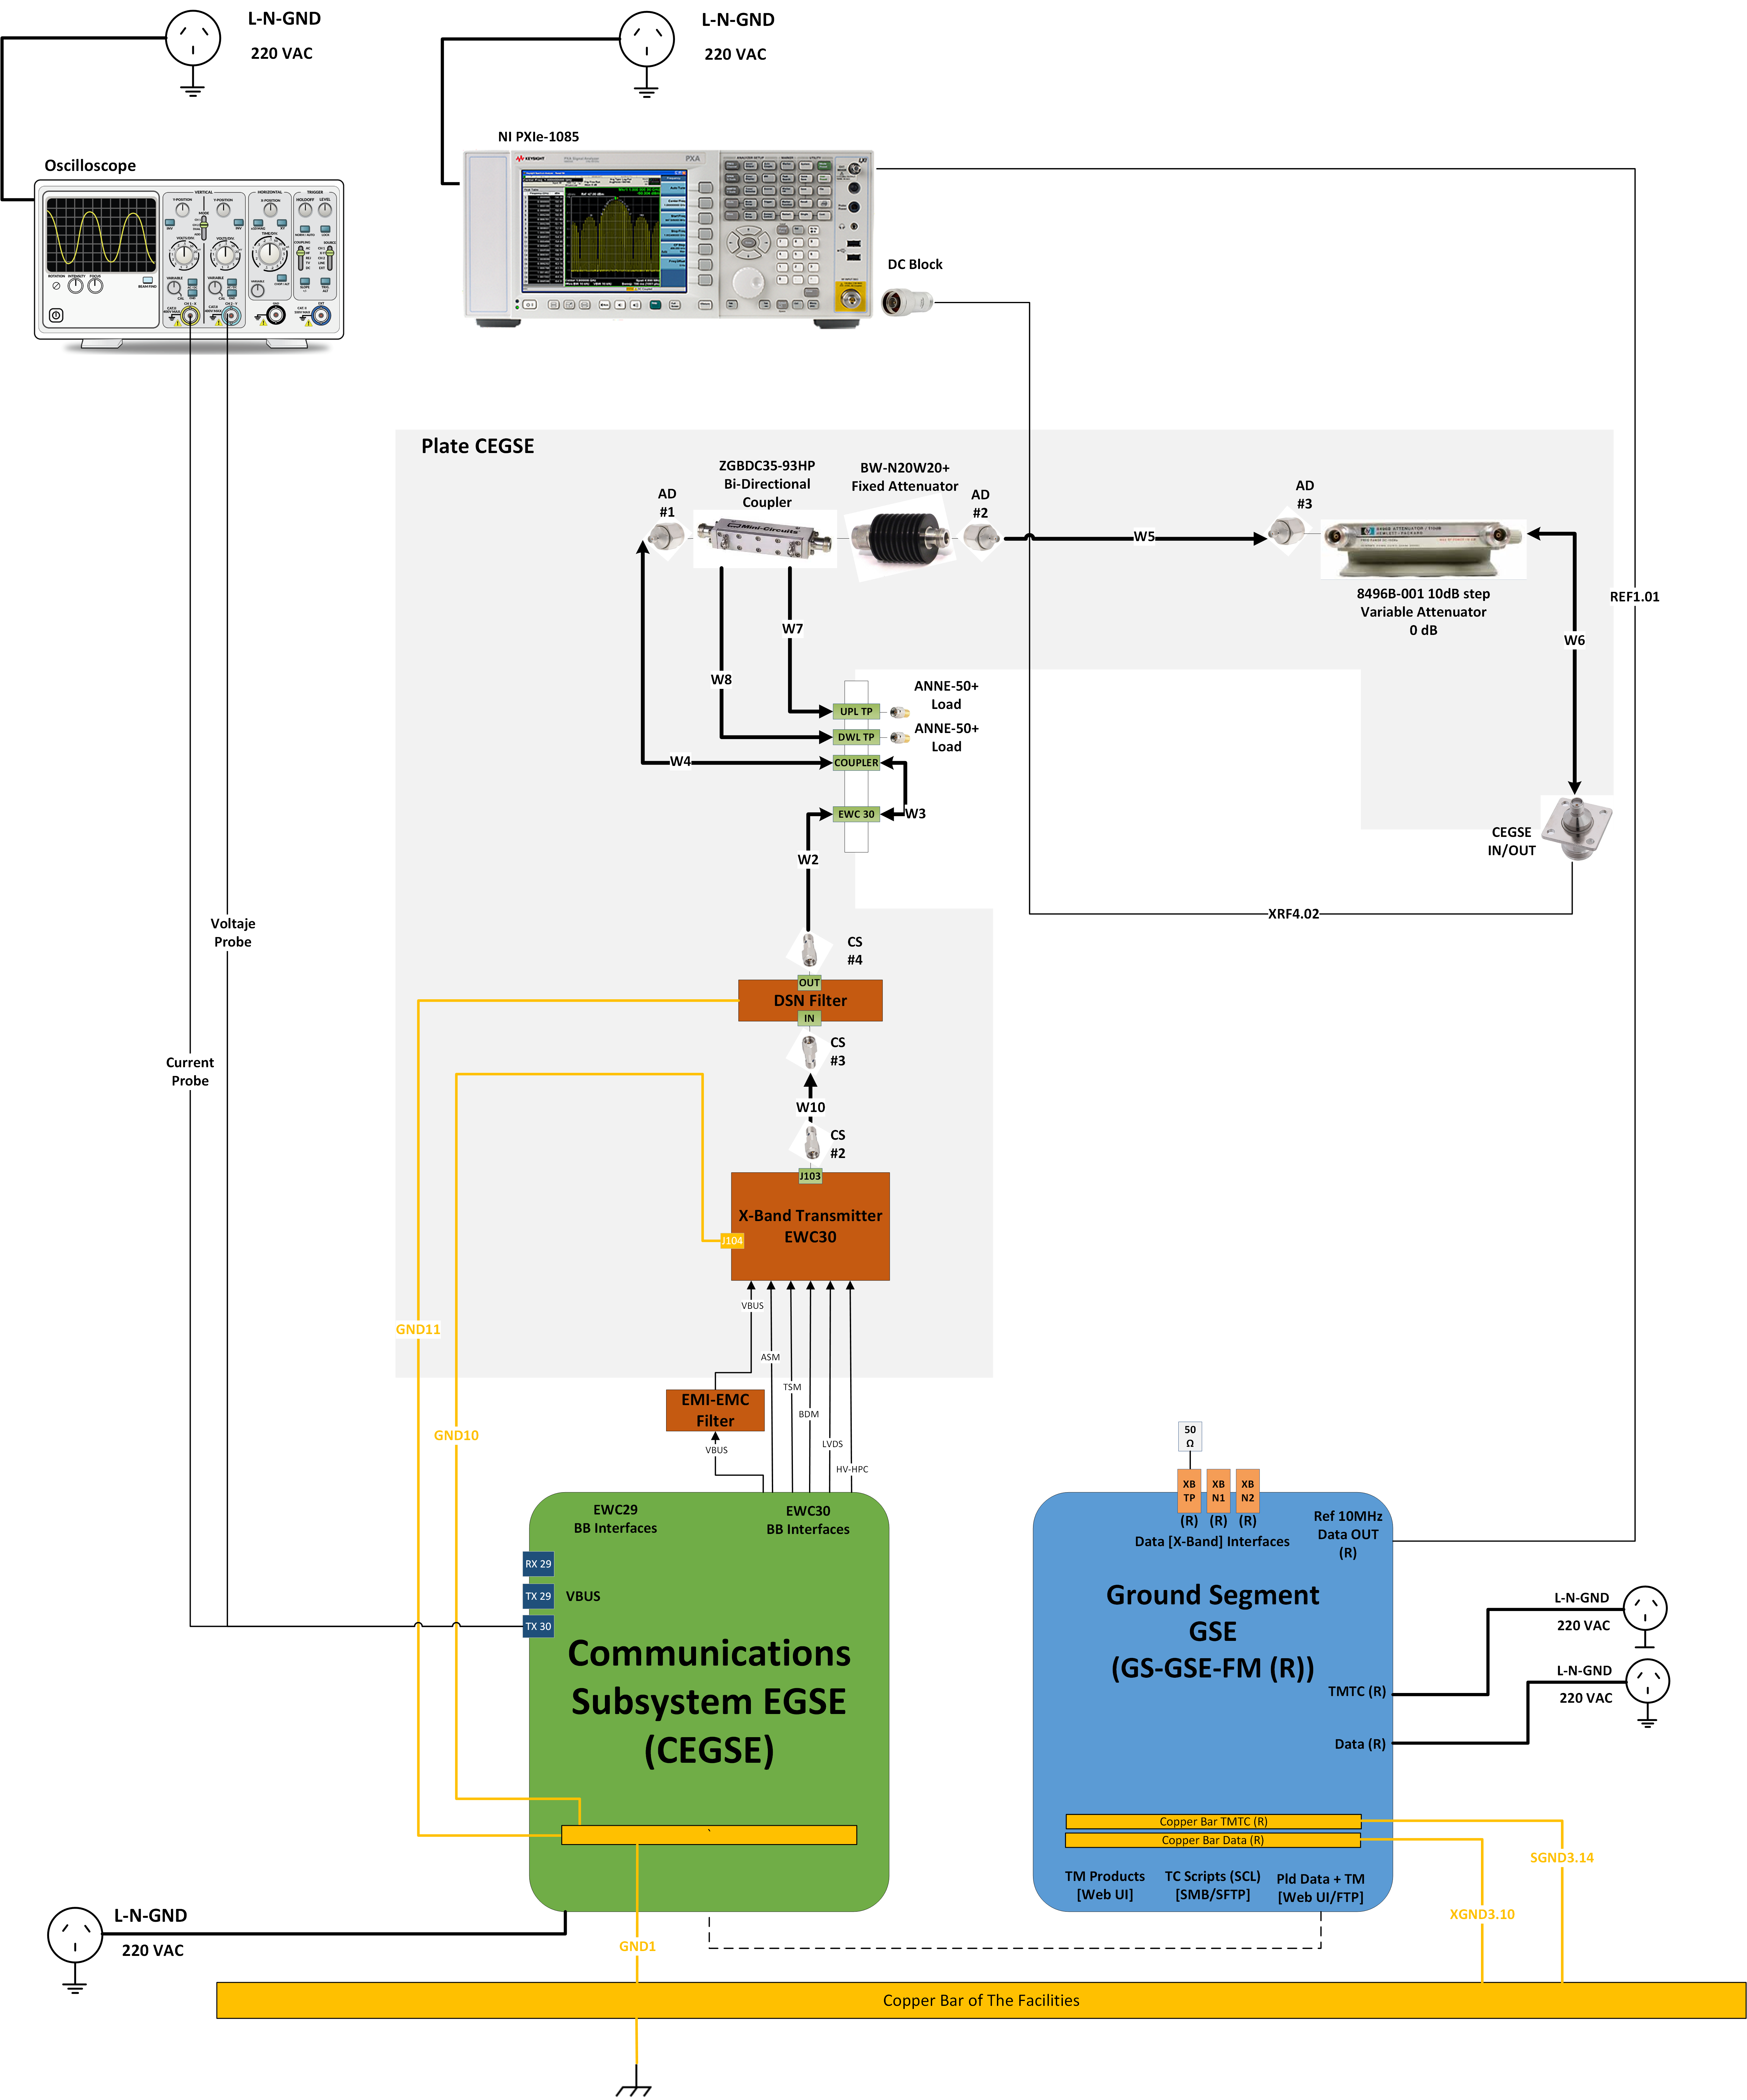
\includegraphics[width=1\linewidth]{figuras/EWC30-PXA-Setup2.png}  
	\caption{EWC30 Spurious in DSN Band Test Setup}
  \label{fig:data-setup2}
\end{figure}
